\documentclass[11pt,a4paper]{article}

\usepackage[T1]{fontenc}
\usepackage{lmodern}
\usepackage[a4paper,margin=21mm,headheight=15pt]{geometry}
\usepackage{microtype}
\usepackage{amsmath,amssymb}
\usepackage{booktabs}
\usepackage{graphicx,float,caption}
\usepackage{xcolor}
\usepackage{fancyhdr}
\usepackage{hyperref}

\definecolor{reportink}{HTML}{163044}
\definecolor{reportaccent}{HTML}{12615E}
\hypersetup{
  colorlinks=true, linkcolor=reportaccent, citecolor=reportaccent, urlcolor=reportaccent,
  pdftitle={Neuronal firing and excitability with the FitzHugh--Nagumo model},
  pdfauthor={Mathematical Modelling Group Project (MAC F314)}
}
\captionsetup{font=small,labelfont={bf,color=reportink},hypcap=false}
\setlength{\parindent}{0pt}
\setlength{\parskip}{0.45em}
\setlength{\emergencystretch}{1em}
\setlength{\tabcolsep}{7pt}

\pagestyle{fancy}
\fancyhf{}
\fancyhead[L]{\small\color{reportink} MAC F314 \enspace|\enspace Mathematical Modelling}
\fancyhead[R]{\small\color{reportink} FitzHugh--Nagumo model}
\fancyfoot[C]{\small\color{reportink}\thepage}
\renewcommand{\headrulewidth}{0.4pt}

\begin{document}

{\color{reportaccent}\small\bfseries MATHEMATICAL MODELLING GROUP PROJECT \enspace MAC F314\par}
\vspace{0.45em}
{\color{reportink}\LARGE\bfseries Neuronal firing and excitability\\[0.15em]
with the FitzHugh--Nagumo model\par}
\vspace{0.35em}
{\large Equilibria, stability, numerical simulation, and sensitivity\par}
% Add the group members' names and roll numbers here for submission.

\vspace{0.7em}
\noindent\textcolor{reportaccent}{\rule{\linewidth}{1pt}}

\subsection*{Abstract}

The FitzHugh--Nagumo model reproduces rest, a single spike, and repeated firing. We derive two equilibrium stability crossings near \(I=0.331\) and \(I=1.419\), where simulations show that the initial state can affect firing. At \(I=0.50\), increasing the recovery rate from \(0.06\) to \(0.10\) shortens the mean period from \(49.157\) to \(33.525\) model time units. From sparse, noisy synthetic voltage, a physics-informed neural network recovered a hidden parameter within \(0.58\%\), compared with \(0.28\%\) for least squares.

\section{Introduction and motivation}

An excitable neuron can respond to a brief electrical disturbance with a rapid voltage spike and then recover. Under a suitable sustained current, it can fire repeatedly. The FitzHugh--Nagumo model represents these responses using a fast voltage variable and a slower recovery variable. Its two-dimensional form allows us to draw the possible states, follow their trajectories, and relate the graphs to equilibrium and stability calculations \cite{fitzhugh1961,nagumo1962}.

\subsection*{Objectives}

\begin{enumerate}
  \item Derive the nullclines and equilibrium equation, and determine local stability from the Jacobian.
  \item Use controlled simulations to compare return to rest, a single spike, and repetitive firing.
  \item Locate current values where the equilibrium changes stability and measure how the recovery parameter affects the interval between spikes.
\end{enumerate}

\section{Assumptions and mathematical formulation}

We model one spatially uniform excitable cell. The state and time are scaled, and the simulations are deterministic. Applied current is constant within each run. A brief nudge is represented as an initial change in voltage while the starting recovery value is fixed. The baseline parameters are \(a=0.7\), \(b=0.8\), and \(\varepsilon=0.08\).

\begin{align}
  \dot v &= v-\frac{v^3}{3}-w+I, \label{eq:voltage}\\
  \dot w &= \varepsilon(v+a-bw). \label{eq:recovery}
\end{align}

Here \(v\) is scaled voltage, \(w\) is the recovery state, \(I\) is the applied current, and a dot denotes differentiation with respect to time. The term \(-w\) lowers the voltage slope as recovery increases. In the second equation, higher \(v\) raises the recovery slope. The small factor \(\varepsilon\) makes recovery evolve more slowly on the time scale of a spike.

\clearpage

\section{Mathematical analysis}

\subsection{Nullclines and equilibria}

A nullcline is a curve on which one rate of change is zero. Setting \(\dot v=0\) gives the cubic voltage nullcline. Setting \(\dot w=0\) gives the straight recovery nullcline.
\begin{equation}
  w=v-\frac{v^3}{3}+I,
  \qquad
  w=\frac{v+a}{b}.
  \label{eq:nullclines}
\end{equation}
An equilibrium is an intersection of these curves, where both rates vanish. Equating the two expressions for \(w\) gives
\begin{equation}
  \frac{b}{3}v_*^3+(1-b)v_*+a-bI=0,
  \qquad
  w_*=\frac{v_*+a}{b}.
  \label{eq:equilibrium}
\end{equation}
The derivative of the cubic with respect to \(v_*\) is \(bv_*^2+1-b>0\) for \(b=0.8\). The cubic is strictly increasing and takes arbitrarily large positive and negative values, so there is exactly one equilibrium at each current. Increasing \(I\) shifts the voltage nullcline upward and moves the equilibrium to a higher voltage.

\subsection{Jacobian and local stability}

The Jacobian records how the two rates respond to small changes in voltage and recovery. At the equilibrium it is
\begin{equation}
  J(v_*)=
  \begin{pmatrix}
    1-v_*^2 & -1\\
    \varepsilon & -\varepsilon b
  \end{pmatrix}.
\end{equation}
Its trace and determinant are
\begin{equation}
  T=1-v_*^2-\varepsilon b,
  \qquad
  D=\varepsilon\bigl[1-b(1-v_*^2)\bigr].
  \label{eq:trace-det}
\end{equation}
The eigenvalues solve \(\lambda^2-T\lambda+D=0\). Negative real parts imply local asymptotic stability. A positive real part implies instability. With our parameters, \(D=\varepsilon(1-b+bv_*^2)>0\), so away from \(T=0\) the sign of the trace determines whether the equilibrium is stable or unstable. The Jacobian predicts the initial response to a small nudge. A larger nudge can explore regions of the phase plane where the linear approximation is inaccurate.

\subsection{Candidate Hopf points}

When \(T=0\) and \(D>0\), the eigenvalues are purely imaginary. Solving \(T=0\) and substituting into \eqref{eq:nullclines} gives
\begin{equation}
  v_H=\pm\sqrt{1-\varepsilon b},
  \qquad
  I_H=\frac{v_H+a}{b}-v_H+\frac{v_H^3}{3}.
  \label{eq:hopf}
\end{equation}
At both candidates \(D=0.075904\). Differentiating \eqref{eq:equilibrium} with respect to \(I\) and using \eqref{eq:trace-det} gives
\begin{equation}
  \frac{dT}{dI}=-\frac{2bv_*}{bv_*^2+1-b}.
\end{equation}
The derivative is about \(+1.631\) at the lower candidate and \(-1.631\) at the upper candidate. The eigenvalue real parts therefore cross zero at a nonzero rate. We use \emph{candidate Hopf point} because the nonlinear coefficient needed to classify the local periodic-orbit bifurcation was left unevaluated \cite{kuznetsov2006}.

\clearpage

\section{Numerical methods}

We solved \eqref{eq:equilibrium} by bisection over \([-3,3]\) for the currents tested, then substituted \((v_*,w_*)\) into both differential equations to check the residuals. We integrated the ODEs with SciPy's \texttt{solve\_ivp} using DOP853, an adaptive Runge--Kutta method \cite{scipy1153}. The relative and absolute tolerances were \(10^{-9}\) and \(10^{-11}\). The initial comparisons report results every \(0.1\) model time units on \([0,150]\). This output grid specifies where values are recorded, while the solver chooses its internal step sizes.

For the displayed firing traces, we counted upward crossings of \(v=0\), estimating each crossing time by linear interpolation between the adjacent output samples. We used the same crossing rule for the sensitivity study. As a numerical check, tightening the sustained-current run to relative and absolute tolerances of \(10^{-11}\) and \(10^{-13}\) changed the sampled states by at most \(4.39\times10^{-8}\).

\section{Simulation results}

\subsection{Small nudge, single spike, and sustained firing}

At \(I=0\), the equilibrium is approximately \((v_*,w_*)=(-1.1994,-0.6243)\). All three experiments start with recovery \(w_*\) from this equilibrium. Table~\ref{tab:runs} gives the initial voltage offsets and the applied currents.

\begin{table}[H]
  \centering
  \caption{Initial voltage offsets from the zero-current equilibrium, applied currents, and observed spike counts on \([0,150]\).}
  \label{tab:runs}
  \begin{tabular}{lrrr}
    \toprule
    Experiment & Voltage offset & Current \(I\) & Spikes\\
    \midrule
    Small nudge    & \(+0.05\) & \(0.00\) & \(0\)\\
    Larger nudge   & \(+0.90\) & \(0.00\) & \(1\)\\
    Sustained input & \(+0.05\) & \(0.50\) & \(4\)\\
    \bottomrule
  \end{tabular}
\end{table}

\begin{figure}[H]
  \centering
  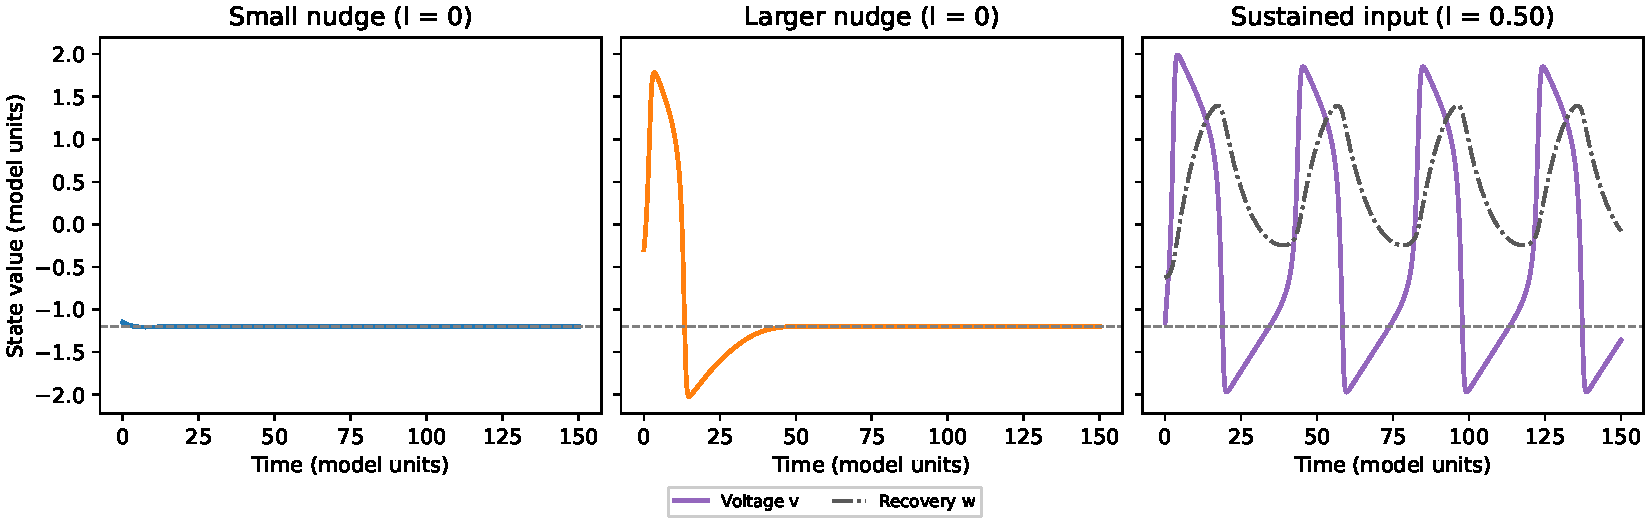
\includegraphics[width=\linewidth]{figures/voltage_responses.pdf}
  \caption{Voltage responses on a common scale. The dashed horizontal line is the zero-current resting voltage. The right panel also shows the slower recovery state.}
  \label{fig:voltage}
\end{figure}

The small nudge decays quickly. The larger nudge gives a single large excursion and returns to the same resting voltage. These two runs have identical parameters and applied current, so their difference demonstrates excitability driven by the initial state. The sustained input keeps producing spikes because it changes the rates at every time during the run.

\clearpage

\subsection{Phase portraits and equilibrium stability}

In the phase plane, the horizontal coordinate is voltage and the vertical coordinate is recovery. At each point, the direction of motion comes from the two rates in \eqref{eq:voltage} and \eqref{eq:recovery}. The arrows in Figure~\ref{fig:phase} are scaled for readability. They show direction, while time plots show the speed of motion.

\begin{figure}[H]
  \centering
  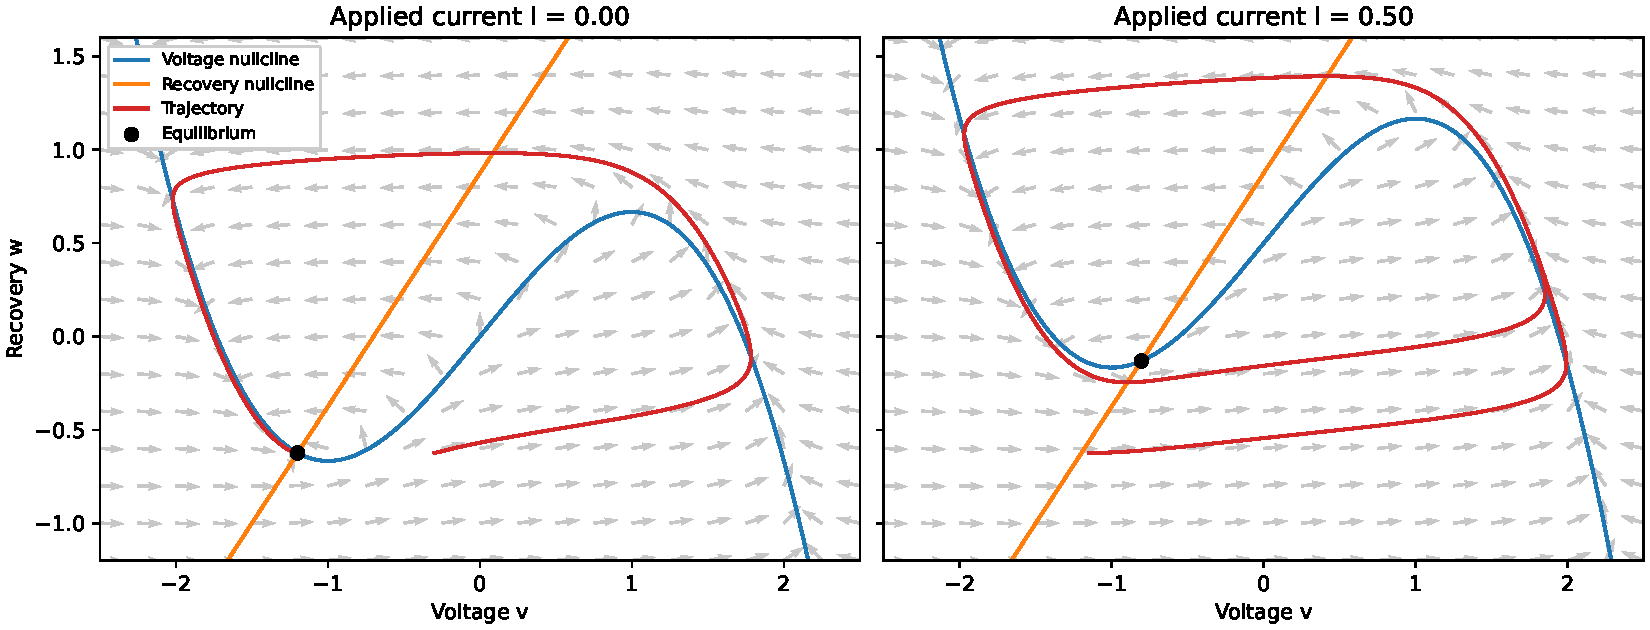
\includegraphics[width=\linewidth]{figures/phase_portraits.pdf}
  \caption{Phase portraits for zero current and \(I=0.50\). The dot in each panel is the equilibrium at the intersection of the nullclines. The red curve shows the trajectory.}
  \label{fig:phase}
\end{figure}

The zero-current trajectory makes a large loop and returns to the equilibrium. With sustained current, the trajectory approaches a repeating loop around the equilibrium. One trip around that loop corresponds to one firing cycle. Both cases have an equilibrium. Their eigenvalues explain why one attracts a small disturbance and the other repels it.

\begin{table}[H]
  \centering
  \caption{Local stability and numerical checks. The initial state is \(0.01\) voltage units from the corresponding equilibrium. The final column gives the Euclidean distance from that equilibrium at time 150.}
  \label{tab:stability}
  \small
  \begin{tabular}{rrrrlr}
    \toprule
    \(I\) & \(v_*\) & \(w_*\) & Eigenvalues & Stability & Final distance\\
    \midrule
    0.00 & \(-1.1994\) & \(-0.6243\) & \(-0.2513\pm0.2119i\) & Stable & \(2.51\times10^{-10}\)\\
    0.50 & \(-0.8048\) & \(-0.1311\) & \(+0.1441\pm0.1915i\) & Unstable & \(1.70\)\\
    1.60 & \(+1.1043\) & \(+2.2554\) & \(-0.1418\pm0.2719i\) & Stable & \(1.41\times10^{-11}\)\\
    \bottomrule
  \end{tabular}
\end{table}

The numerical perturbation checks agree with the eigenvalues at all three currents. At \(I=1.60\), the equilibrium is locally stable again, at a higher voltage than the zero-current resting state. At \(I=0.50\), the positive real parts predict initial growth of a small disturbance. The large, bounded oscillation that follows is a property of the nonlinear system seen in the simulation.

\clearpage

\subsection{Current sweep and behaviour near the crossings}

We varied \(I\) from 0 to 1.75 in increments of 0.025, using the same initial state as the small-nudge experiment in Table~\ref{tab:runs}. For each run, we recorded the minimum and maximum voltage over \([300,600]\), sampled every \(0.2\) time units. Figure~\ref{fig:sweep} compares these extrema with the equilibrium voltage and the largest eigenvalue real part. The dotted lines mark the two analytically located crossings, \(I\approx0.331281\) and \(1.418719\).

\begin{figure}[H]
  \centering
  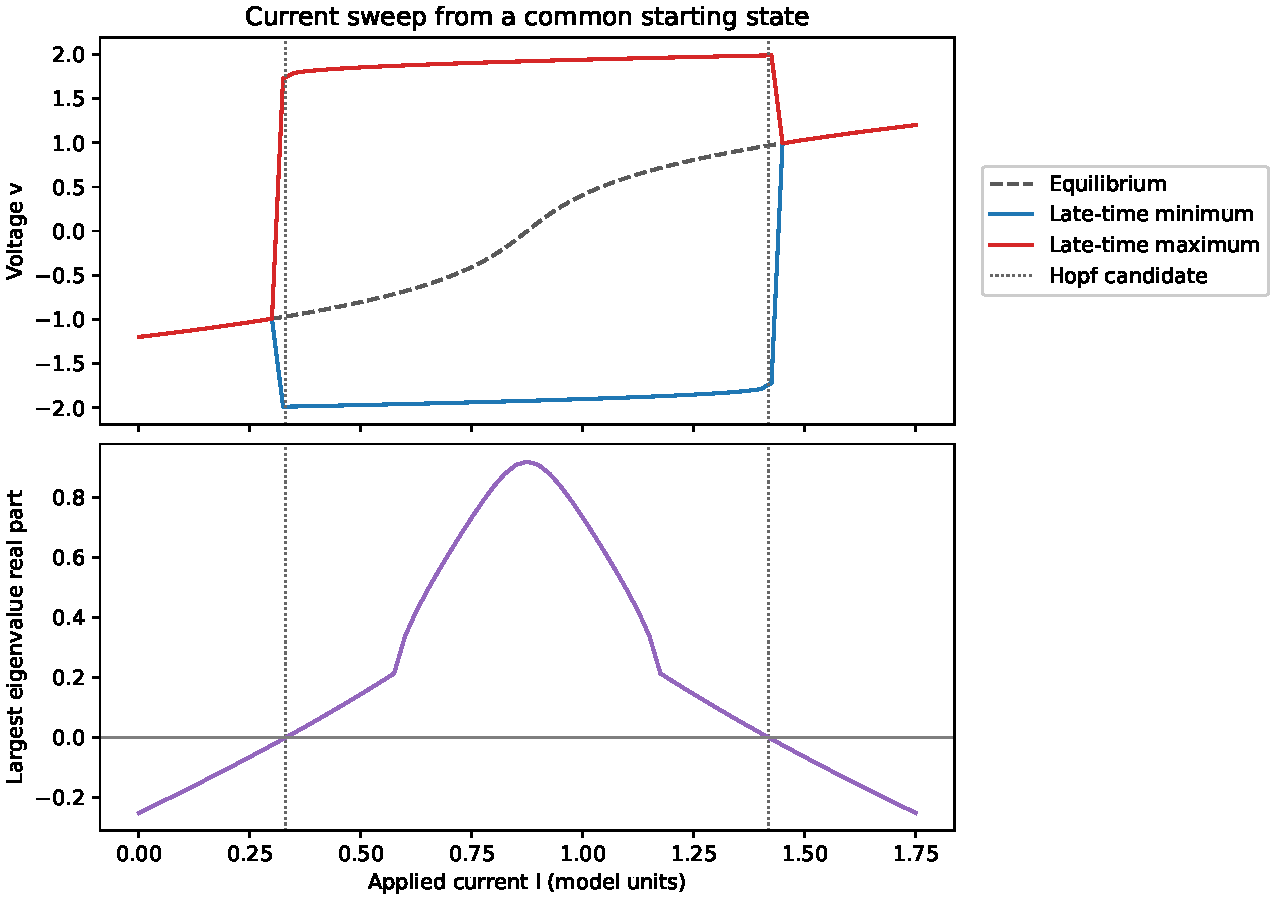
\includegraphics[width=0.83\linewidth]{figures/current_sweep.pdf}
  \caption{The upper panel shows equilibrium voltage and late-time extrema from a common initial state. The lower panel shows the largest eigenvalue real part.}
  \label{fig:sweep}
\end{figure}

We also simulated currents \(0.004\) below and above each candidate. Each run started at the corresponding equilibrium recovery value, with voltage nudged toward the middle of the voltage range by either \(0.01\) or \(0.80\). Table~\ref{tab:refined} shows the resulting voltage span, maximum minus minimum, on \([1700,2000]\).

\begin{table}[H]
  \centering
  \caption{Refined simulations near the stability crossings. A span close to zero indicates a trajectory that has nearly settled over the recorded window.}
  \label{tab:refined}
  \small
  \begin{tabular}{rrrr}
    \toprule
    \(I\) & Largest real part & Span after \(0.01\) nudge & Span after \(0.80\) nudge\\
    \midrule
    0.327281 & \(-0.00326\) & 0.00008 & 3.73783\\
    0.335281 & \(+0.00327\) & 3.76057 & 3.76057\\
    1.414719 & \(+0.00327\) & 3.76057 & 3.76057\\
    1.422719 & \(-0.00326\) & 0.00008 & 3.73783\\
    \bottomrule
  \end{tabular}
\end{table}

At the two tested currents on the stable sides, the small nudge nearly settles and the larger nudge keeps oscillating over the late window. This is numerical evidence consistent with coexistence of a stable equilibrium and a firing state for those settings. The finite windows and the tested starting states limit the strength and range of that conclusion.

\clearpage

\subsection{Sensitivity to the recovery rate}

With \(I=0.50\) and the same starting state, we changed only \(\varepsilon\). We simulated to time 450, recorded output every \(0.1\) time units, and discarded spike crossings before time 150. The mean period is the average time between successive retained crossings.

\begin{center}
  \begin{minipage}[c]{0.55\linewidth}
    \centering
    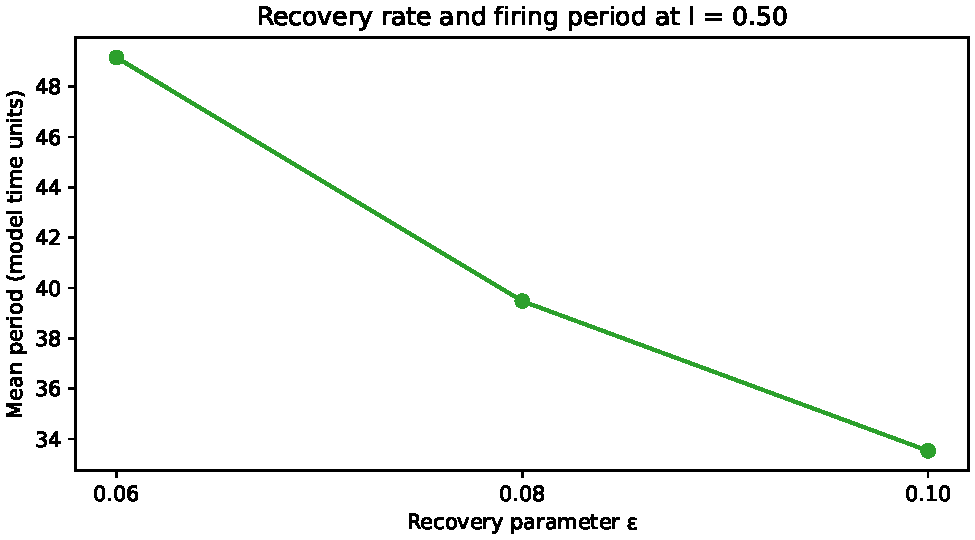
\includegraphics[width=\linewidth]{figures/recovery_sensitivity.pdf}
    \captionof{figure}{Mean firing period at \(I=0.50\).}
    \label{fig:sensitivity}
  \end{minipage}\hfill
  \begin{minipage}[c]{0.42\linewidth}
    \centering
    \captionof{table}{Recovery sensitivity. Periods are in model time units.}
    \label{tab:sensitivity}
    \small
    \begin{tabular}{@{}rrr@{}}
      \toprule
      \(\varepsilon\) & Late spikes & Mean period\\
      \midrule
      0.06 & 7 & 49.157\\
      0.08 & 8 & 39.475\\
      0.10 & 9 & 33.525\\
      \bottomrule
    \end{tabular}
  \end{minipage}
\end{center}

Faster recovery reduced the average interval between spikes across the tested range. The mean period decreased by about \(32\%\) between the first and last settings. This comparison describes one current and three recovery settings.

\section{Bonus study of parameter estimation with a PINN}
\label{sec:bonus}

\subsection{Inverse problem and synthetic data}

The core simulations use known parameters to predict voltage. Here we reverse the problem and estimate \(a\) from voltage readings alone. We fix \(b=0.80\) and \(\varepsilon=0.08\), supply the current and initial state, and treat recovery \(w\) as unobserved during fitting. The data come from the FHN equations with \(a_{\mathrm{true}}=0.70\), so the parameter error can be measured directly.

We generated clean reference trajectories on \([0,40]\) at intervals of \(0.10\), using DOP853 with relative and absolute tolerances of \(10^{-11}\) and \(10^{-13}\). For the clean training set, we kept every fourth voltage sample, giving 101 observations. For the sparse, noisy set, we chose one positive-time sample per block of ten and added Gaussian noise with standard deviation \(0.03\), giving 40 observations. The two sets sample the same training trajectory.

Training used \(I=0.50\) and \((v_0,w_0)=(-1.15,-0.62)\). Validation used \(I=0.65\) and \((-1.00,-0.55)\). The final test used \(I=0.90\) and \((-1.20,-0.70)\). Only training observations entered either fit.

\begin{figure}[H]
  \centering
  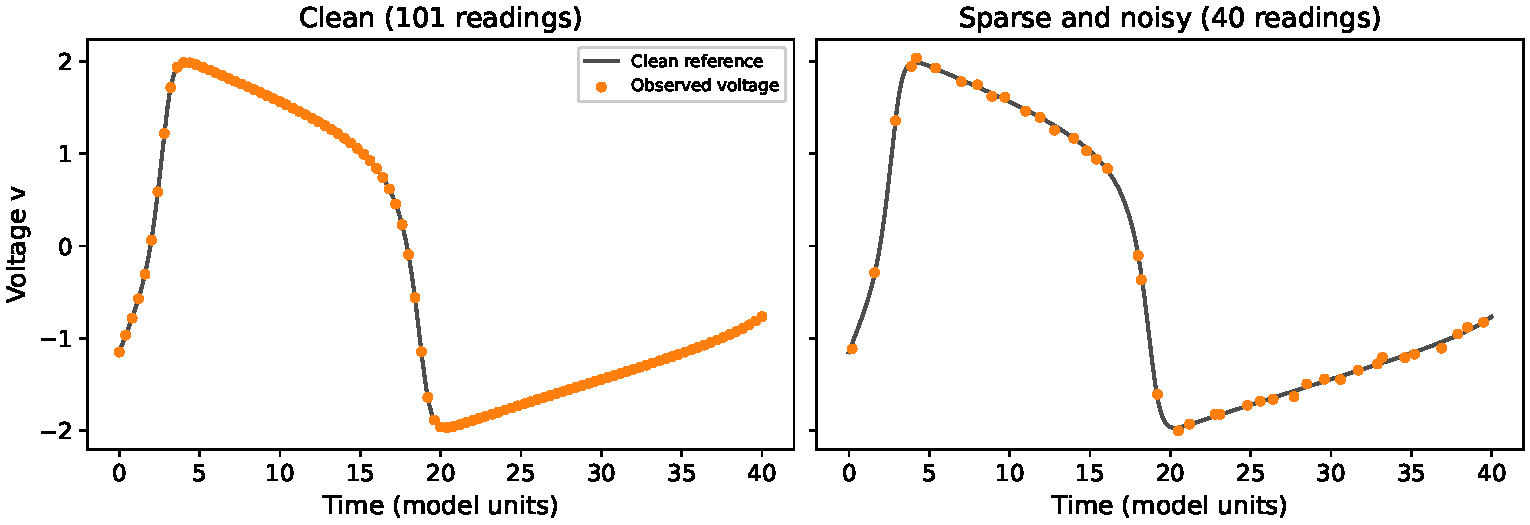
\includegraphics[width=0.83\linewidth]{figures/pinn_training_observations.pdf}
  \caption{The two training datasets. Dots are the supplied observations and the gray curve is the clean numerical reference.}
  \label{fig:pinn-data}
\end{figure}

\clearpage

\subsection{PINN and least-squares fitting}

A physics-informed neural network (PINN) fits observed data while penalizing disagreement with the governing equations \cite{raissi2019}. Our network takes time as input and predicts voltage \(\hat v\) and recovery \(\hat w\). It uses normalized time, three pairs of sine and cosine features, and three hidden layers of 32 units with \(\tanh\) activations. The output takes the form \((\hat v,\hat w)=(v_0,w_0)+(1-e^{-t})N_\theta(t)\), which gives the known initial state exactly at \(t=0\).

At 241 fixed physics times, automatic differentiation supplies the predicted slopes. The residuals are the predicted slopes minus the rates from \eqref{eq:voltage} and \eqref{eq:recovery}, evaluated at the predicted state and fitted \(\hat a\). The objective is
\begin{equation}
  \mathcal{L}
  =\operatorname{mean}_{\rm obs}\!\bigl[(\hat v-v_{\rm obs})^2\bigr]
    +\operatorname{mean}_{\rm grid}\!\bigl[r_v^2+4r_w^2\bigr].
  \label{eq:pinn-loss}
\end{equation}
On a Colab CPU in double precision, we used 400 voltage-only steps, 1800 joint Adam steps, and up to 300 L-BFGS iterations. The data seed was 2026 and the network seed was 7.

The least-squares baseline integrates the FHN model for each trial \(a\) and minimizes squared voltage errors at the same observation times. Both fits start at \(a=0.50\) with the same allowed interval \([0.20,1.20]\).

\subsection{Held-out results}

For validation and testing, we used each fitted \(a\) in the same numerical ODE solver at the new current and initial state. This checks parameter transfer to another trajectory. The voltage error is the root mean square error (RMSE) against the corresponding clean reference. Relative parameter error is \(100|\hat a-a_{\mathrm{true}}|/|a_{\mathrm{true}}|\).

\begin{table}[H]
  \centering
  \caption{Parameter recovery and final-test errors at \(I=0.90\). Entries shown as zero are rounded to the displayed precision.}
  \label{tab:pinn-test}
  \small
  \setlength{\tabcolsep}{5pt}
  \begin{tabular}{llrrrr}
    \toprule
    Training data & Method & \(\hat a\) & Rel.\ error & Voltage RMSE & Recovery RMSE\\
    \midrule
    Clean & PINN          & 0.699975 & \(0.0036\%\) & 0.000096 & 0.000022\\
    Clean & Least squares & 0.700000 & \(0.00\%\)   & 0.000000 & 0.000000\\
    Sparse, noisy & PINN          & 0.704093 & \(0.58\%\) & 0.015570 & 0.003554\\
    Sparse, noisy & Least squares & 0.701926 & \(0.28\%\) & 0.007343 & 0.001677\\
    \bottomrule
  \end{tabular}
\end{table}

\begin{figure}[H]
  \centering
  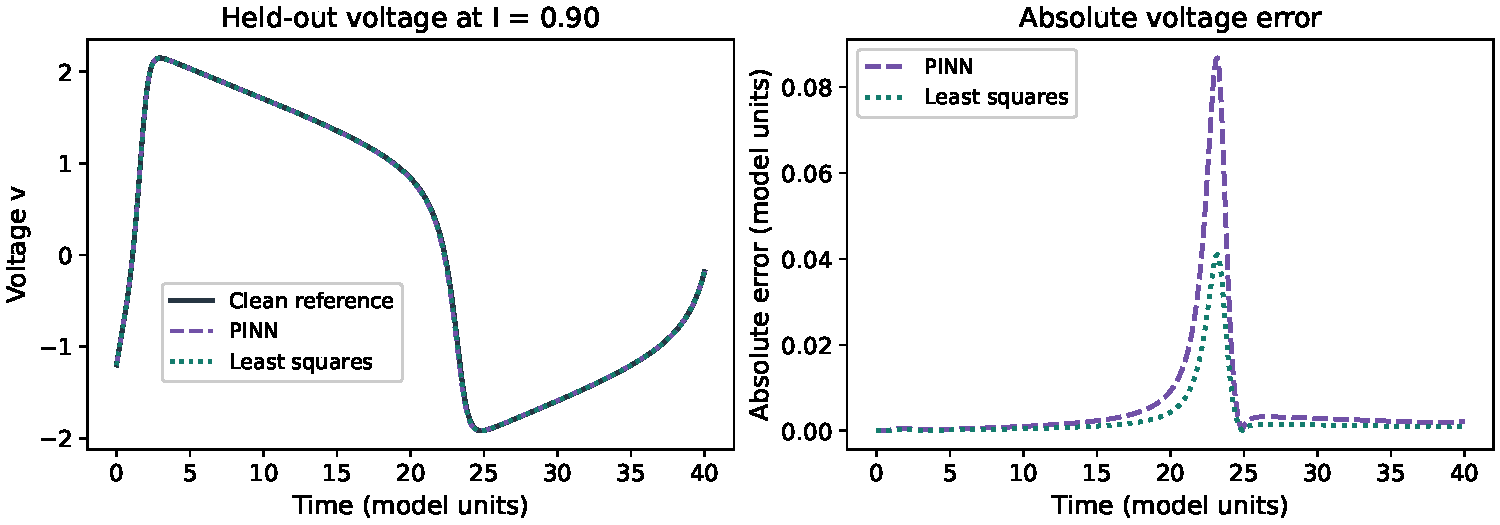
\includegraphics[width=0.91\linewidth]{figures/pinn_heldout_comparison.pdf}
  \caption{Final-test voltages and absolute errors for the sparse, noisy fits. The curves are regenerated from the fitted parameters rounded to six decimal places.}
  \label{fig:pinn-test}
\end{figure}

Both methods matched the single reference spike in the final test. On noisy validation data, voltage RMSE was \(0.011649\) for the PINN and \(0.005491\) for least squares.


\clearpage

\section{Conclusion and limitations}

The FitzHugh--Nagumo model reproduced three distinct responses by changing the initial voltage or the sustained current. Equilibrium and Jacobian calculations explained when small disturbances decayed or grew. The current sweep identified two stability crossings, and the refined runs showed that the initial state can matter near a crossing. At the tested current, increasing the recovery rate shortened the firing period.

The variables are scaled, so comparing the curves to a particular neuron would require calibration against measured voltage, time, and current. The late-time simulations sample selected currents and initial states. A full description of periodic branches and their stability would require additional analysis. The core Jupyter notebook regenerates the simulations and exports the core figures.

In the bonus experiment, both methods recovered the true \(a\) within \(1\%\) from sparse, noisy voltage and transferred the estimate to a different current and starting state. Least squares had lower parameter and trajectory errors in this experiment, where the forward model was known. The comparison between the clean and noisy sets combines a change in sample density with added noise. Because the benchmark uses one synthetic model, one observation seed, and one network seed, it measures recovery under these controlled assumptions. Estimating additional parameters or comparing against a real recording would require further experiments.

\subsection*{Reproducibility}

The executed Colab notebook contains the training logs, fitted values, validation and final-test tables, and comparison plots. The run used PyTorch 2.14.1, SciPy 1.16.3, and Matplotlib 3.10.0. See the \href{https://github.com/Rigur-Calypso/Mathematical-Modelling-Group-Project-MAC-F314/blob/e78813a679367d4be962c1d8b4448c56e6846b50/fhn_pinn_ml.ipynb}{executed PINN notebook}.

\begingroup
\small
\setlength{\parskip}{0pt}
\bibliographystyle{unsrt}
\bibliography{references}
\endgroup

\end{document}
